\documentclass{beamer}

\usepackage{verbatim}
\usepackage{fancyvrb}
\usepackage{amsmath}
\usepackage{mathtools}
\usepackage{booktabs}
\usepackage{amssymb}
\usepackage{graphicx}
\usepackage{calc}
\usepackage{color}
\usepackage{multicol}
\usepackage{wrapfig}
\usepackage{natbib}
\usepackage[ruled,vlined]{algorithm2e}
\usepackage{animate}
\usepackage{mathtools}
\usepackage{listings}

\usepackage{cmbright}
\fontencoding{OT1}\fontfamily{cmbr}\selectfont %to load ot1cmbr.fd
\DeclareFontShape{OT1}{cmbr}{bx}{n}{% change bx definition
<->cmbrbx10%
}{}
\normalfont % back to normalfont

% two col: two columns
\newenvironment{twocol}[4]{
\begin{columns}[c]
\column{#1\textwidth}
#3
\column{#2\textwidth}
#4
\end{columns}
}

\makeatletter
\setbeamertemplate{theorem begin}
{%
\begin{\inserttheoremblockenv}
  {}{\usebeamerfont*{block title}\usebeamercolor[fg]{block title}%
  \inserttheoremname
  %\inserttheoremnumber
  \ifx \inserttheoremaddition \empty \else\ (\inserttheoremaddition)\fi
  \inserttheorempunctuation}
  \normalfont
  }
  \setbeamertemplate{theorem end}{\end{\inserttheoremblockenv}}
\makeatother

\newcommand{\E}{\mathrm{E}}
\newcommand{\Var}{\mathrm{Var}}
\newcommand{\Cov}{\mathrm{Cov}}
\newcommand{\sd}{\mathrm{sd}}
\newcommand{\se}{\mathrm{se}}
\newcommand{\Corr}{\mathrm{Corr}}
\newcommand{\rank}{\mathrm{rank}}
\newcommand{\trace}{\mathrm{trace}}
\newcommand{\nullspace}{\mathrm{null}}
\newcommand{\myspan}{\mathrm{span}}
\DeclareMathOperator*{\argmax}{arg\,max}
\DeclareMathOperator*{\argmin}{arg\,min}
\DeclareMathOperator*{\softmax}{softmax}

\definecolor{darkgreen}{rgb}{0,0.5,0}

\newtheorem{proposition}[theorem]{Proposition}
\newtheorem{exe}{Exercise}
\newtheorem{notation}{Notation}
\newtheorem{remark}{Remark}

\definecolor{darkgreen}{rgb}{0,0.5,0}

\title{Matrix Approach to SLR}
\author{Zhenisbek Assylbekov}
\institute{Department of Mathematics}
\date{Regression Analysis}

\AtBeginSection[]
{
  \begin{frame}<beamer>
    \tableofcontents[currentsection]
  \end{frame}
}

\begin{document}

\begin{frame}
  \titlepage
\end{frame}

\section{Random Vectors}

\begin{frame}{Random Vectors}
Let $\mathbf{Y}$ be a random vector in $\mathbb{R}^n$, i.e.
$$
\mathbf{Y}=\begin{bmatrix}
Y_1\\
\vdots\\
Y_n
\end{bmatrix}
$$
\pause The \textbf{pdf} of $\mathbf{Y}$ is the joint pdf of $Y_1,\ldots,Y_n$:
$$
f_{\mathbf{Y}}(\mathbf{y})=f_{Y_1,\ldots,Y_n}(y_1,\ldots,y_n)
$$
\pause It is a function s.t. for any (measurable) $B\subset\mathbb{R}^n$:
\begin{align*}
\Pr(\mathbf{Y}\in B)&=\int_{\mathbf{y}\in B}f_{Y_1,\ldots,Y_n}(y_1,\ldots,y_n)dy_1\cdots d y_n\\
\onslide<4->{&=\int_{\mathbf{y}\in B}f_\mathbf{Y}(\mathbf{y})d\mathbf{y}}
\end{align*}
\end{frame}

\begin{frame}{Expectation of a Random Vector}
The \textbf{expectation} of a random vector $\mathbf{Y}$ is
$$
\boldsymbol\mu=\E[\mathbf{Y}]=\begin{bmatrix}
\E[Y_1]\\
\vdots\\
\E[Y_n]
\end{bmatrix}
$$
\end{frame}

\begin{frame}{Random Vectors}
The \textbf{covariance matrix} of a random vector $\mathbf{Y}$ is an $n\times n$ matrix defined as
\begin{footnotesize}
\begin{align*}
\Var[\mathbf{Y}]&=\E[(\mathbf{Y}-\E[\mathbf{Y}])(\mathbf{Y}-\E[\mathbf{Y}])^\top]\\
\onslide<2->{&=\begin{bmatrix}
\Var[Y_1] & \Cov[Y_1,Y_2] & \cdots & \Cov[Y_1,Y_n] \\
\Cov[Y_2,Y_1] & \Var[Y_2] & \cdots & \Cov[Y_2,Y_n]\\
\vdots & \vdots & \ddots & \vdots \\
\Cov[Y_n,Y_1] & \Cov[Y_n,Y_2] & \cdots & \Var[Y_n]
\end{bmatrix}\\}
\onslide<3->{&=
\begin{bmatrix}
\sigma_1^2 & \sigma_{1,2} & \cdots & \sigma_{1,n}\\
\sigma_{2,1} & \sigma_{2}^2 & \cdots & \sigma_{2,n}\\
\vdots & \vdots & \ddots & \vdots \\
\sigma_{n,1} & \sigma_{n,2} & \cdots & \sigma_{n}^2
\end{bmatrix}\\}
\onslide<4->{&=\boldsymbol\Sigma\qquad\text{(symmetric)}}
\end{align*}
\end{footnotesize}
\end{frame}

\begin{frame}{SLR}
In the regression model, the only random term is $\boldsymbol\epsilon$ with
$$
\E[\boldsymbol\epsilon]=\pause\begin{bmatrix}
0\\
\vdots\\
0
\end{bmatrix}=\mathbf{0}\quad\text{and}\quad\Var[\boldsymbol\epsilon]\pause=\begin{bmatrix}
\sigma^2 & 0 & \cdots & 0\\
0 & \sigma^2 & \cdots & 0\\
\vdots & \vdots & \ddots & \vdots\\
0 & 0 & \cdots & \sigma^2
\end{bmatrix}=\sigma^2\mathbf{I}_n
$$
\pause Hence for the model
$$
\mathbf{Y}=\mathbf{X}\boldsymbol\beta+\boldsymbol\epsilon
$$
\begin{itemize}
    \item\pause $\E[\mathbf{Y}]\pause=\E[\mathbf{X}\boldsymbol\beta]+\E[\boldsymbol\epsilon]=\mathbf{X}\boldsymbol\beta$
    \item\pause $\Var[\mathbf{Y}]\pause=\Var[\mathbf{X}\boldsymbol\beta+\boldsymbol\epsilon]=\Var[\boldsymbol\epsilon]=\sigma^2\mathbf{I}_n$
\end{itemize}
\end{frame}

\begin{frame}{Linear Transform of a Random Vector}
Let $\mathbf{A}\in\mathbb{R}^{m\times n}$ and $\mathbf{Y}$ be a random $n$-vector, then
\begin{align*}
\mathbf{AY}&=\onslide<2->{\begin{bmatrix}
a_{11} & a_{12} & \cdots & a_{1n}\\
a_{21} & a_{22} & \cdots & a_{2n}\\
\vdots & \vdots & \ddots & \vdots\\
a_{m1} & a_{m2} & \cdots & a_{mn}
\end{bmatrix}\begin{bmatrix}
Y_1\\
Y_2\\
\vdots\\
Y_n
\end{bmatrix}\\}
\onslide<3->{&=\begin{bmatrix}
a_{11}Y_1+a_{12}Y_2+\ldots+a_{1n}Y_n\\
a_{21}Y_1+a_{22}Y_2+\ldots+a_{2n}Y_n\\
\vdots\\
a_{m1}Y_1+a_{m2}Y_2+\ldots+a_{mn}Y_n
\end{bmatrix}}
\end{align*}
\end{frame}


\begin{frame}{Mean of a Linear Transform}
\begin{theorem}
Let $\mathbf{Y}$ be a random $n$-vector, and $\mathbf{A}\in\mathbb{R}^{m\times n}$. Then $\E[\mathbf{AY}]=\mathbf{A}\E[\mathbf{Y}]$.
\end{theorem}
\begin{proof}
\begin{footnotesize}
\begin{align*}
\E[\mathbf{AY}]&=\onslide<2->{\begin{bmatrix}
\E[a_{11}Y_1+a_{12}Y_2+\ldots+a_{1n}Y_n]\\
\vdots\\
\E[a_{m1}Y_1+a_{m2}Y_2+\ldots+a_{mn}Y_n]
\end{bmatrix}\\}
\onslide<3->{&=\begin{bmatrix}
a_{11}\E[Y_1]+a_{12}\E[Y_2]+\ldots+a_{1n}\E[Y_n]\\
\vdots\\
a_{m1}\E[Y_1]+a_{m2}\E[Y_2]+\ldots+a_{mn}\E[Y_n]
\end{bmatrix}\\}
\onslide<4->{&=\begin{bmatrix}
a_{11} & a_{12} & \cdots & a_{1n}\\
a_{21} & a_{22} & \cdots & a_{2n}\\
\vdots & \vdots & \ddots & \vdots\\
a_{m1} & a_{m2} & \cdots & a_{mn}
\end{bmatrix}\begin{bmatrix}
\E[Y_1]\\
\E[Y_2]\\
\vdots\\
\E[Y_n]
\end{bmatrix}\\}
\onslide<5->{&=\mathbf{A}\E[\mathbf{Y}]}
\end{align*}
\end{footnotesize}
\end{proof}
\end{frame}

\begin{frame}{Covariance Matrix of a Linear Transform}
\begin{theorem}
Let $\mathbf{Y}$ be a random $n$-vector, and $\mathbf{A}\in\mathbb{R}^{m\times n}$. Then $\Var[\mathbf{AY}]=\mathbf{A}\Var[\mathbf{Y}]\mathbf{A}^\top$.
\end{theorem}
\begin{proof}
\begin{align*}
\Var[\mathbf{AY}]&=\onslide<2->{\E[(\mathbf{AY}-\E[\mathbf{AY}])(\mathbf{AY}-\E[\mathbf{AY}])^\top]\\}
\onslide<3->{&=\E[(\mathbf{AY}-\mathbf{A}\E[\mathbf{Y}])(\mathbf{AY}-\mathbf{A}\E[\mathbf{Y}])^\top]\\}
\onslide<4->{&=\E[\mathbf{A}(\mathbf{Y}-\E[\mathbf{Y}])(\mathbf{Y}-\E[\mathbf{Y}])^\top\mathbf{A}^\top]\\}
\onslide<5->{&=\mathbf{A}\E[(\mathbf{Y}-\E[\mathbf{Y}])(\mathbf{Y}-\E[\mathbf{Y}])^\top]\mathbf{A}^\top\\}
\onslide<6->{&=\mathbf{A}\Var[\mathbf{Y}]\mathbf{A}^\top}
\end{align*}    
\end{proof}
\end{frame}

\begin{frame}{Covariance Matrix is Positive Semi-definite}
\begin{theorem}
Let $\mathbf{Y}$ be a random vector in $\mathbb{R}^n$. Then $\Var[\mathbf{Y}]\succeq\mathbf{0}$.
\end{theorem}
\pause\begin{proof}
$\forall\mathbf{a}\in\mathbb{R}^n$:
$$
\mathbf{a}^\top\Var[\mathbf{Y}]\mathbf{a}\pause=\Var[\mathbf{a}^\top\mathbf{Y}]\pause\ge0,
$$ 
since $\mathbf{a}^\top\mathbf{Y}=\sum_i a_iY_i$ is a random variable with values in $\mathbb{R}^1$.
\end{proof}
\end{frame}

\begin{frame}{Pdf of a Linear Transform, $n=1$}
\begin{theorem}
Let $X$ be a continuous r.v. with the pdf $f_X(x)$, and $a\ne0$. Then the pdf of $Y=aX$ is given by
$$
f_{Y}(y)=\frac{1}{|a|}f_X\left(\frac{y}{a}\right)
$$
\end{theorem}
\begin{proof}
For $a>0$:
\begin{align*}
f_Y(y)&\onslide<2->{=\frac{d}{dy}[F_Y(y)]}\onslide<3->{=\frac{d}{dy}\left[\Pr(Y\le y)\right]}\onslide<4->{=\frac{d}{dy}\left[\Pr(aX\le y\right]\\}
\onslide<5->{&=\frac{d}{dy}\left[\Pr\left(X\le\frac{y}{a}\right)\right]}\onslide<6->{=\frac{d}{dy}\left[F_X\left(\frac{y}{a}\right)\right]}\onslide<7->{=\frac1a f_X\left(\frac{y}{a}\right)}
\end{align*}
\onslide<8->{For $a<0$ the proof is analogous and is left as \textit{exercise}.}
\end{proof}
\end{frame}

\begin{frame}{Pdf of a Linear Transform, General Case}
\begin{theorem}
Let $\mathbf{X}$ be a random vector with the pdf $f_{\mathbf{X}}(\mathbf{x})$, and $\mathbf{A}\in\mathbb{R}^{n\times n}$ with $\det\mathbf{A}\ne0$. Then the pdf of $\mathbf{Y}=\mathbf{AX}$ is given by
$$
f_{\mathbf{Y}}(\mathbf{y})=\frac{1}{|\det\mathbf{A}|}f_\mathbf{X}(\mathbf{A}^{-1}\mathbf{y})
$$
\end{theorem}
\pause\begin{proof} For any $B\subset \mathbb{R}^n$,
\begin{align*}
\onslide<3->{\int_{\mathbf{y}\in B}f_{\mathbf{Y}}(\mathbf{y})d\mathbf{y}=\Pr(\mathbf{Y}\in B)&}\onslide<4->{=\Pr(\mathbf{AX}\in B)}\onslide<5->{=\int_{\mathbf{Ax}\in B}f_\mathbf{X}(\mathbf{x})d\mathbf{x}\\}
\onslide<6->{&=\int_{\mathbf{y}\in B}f_{\mathbf{X}}(\mathbf{A}^{-1}\mathbf{y})|\det\mathbf{A}^{-1}|d\mathbf{y}}
\end{align*}
\onslide<7->{Noting that $\det\mathbf{A}^{-1}=\frac{1}{\det\mathbf{A}}$ concludes the proof.}
\end{proof}
\end{frame}

\begin{frame}{Pdf of an Affine Transform}
\begin{theorem}
Let $X$ be a continuous r.v. with the pdf $f_X(x)$, and $a\ne0$. Then the pdf of $Y=aX+b$ is given by
$$
f_{Y}(y)=\frac{1}{|a|}f_X\left(\frac{y-b}{a}\right)
$$
\end{theorem}

\pause\begin{theorem}
Let $\mathbf{X}$ be a random vector with the pdf $f_{\mathbf{X}}(\mathbf{x})$, $\mathbf{A}\in\mathbb{R}^{n\times n}$ with $\det\mathbf{A}\ne0$, and $\mathbf{b}\in\mathbb{R}^b$. Then the pdf of $\mathbf{Y}=\mathbf{AX}+\mathbf{b}$ is given by
$$
f_{\mathbf{Y}}(\mathbf{y})=\frac{1}{|\det\mathbf{A}|}f_\mathbf{X}(\mathbf{A}^{-1}(\mathbf{y}-\mathbf{b}))
$$
\end{theorem}

\pause \begin{proof}[Proofs are left as exercises]\end{proof}
\end{frame}


\section{Multivariate Gaussian Distribution}

\begin{frame}{Multivariate Normal Distribution}
\begin{definition}
A random vector $\mathbf{Y}=\begin{bmatrix}Y_1 & \ldots & Y_n\end{bmatrix}^\top$ is \textbf{multivariate normal (Gaussian)} if
it can be represented as
$$
\mathbf{Y}=\mathbf{AZ}+\boldsymbol{\mu},
$$
where 
\begin{itemize}
    \item $\mathbf{Z}=\begin{bmatrix}Z_1 & \ldots & Z_k\end{bmatrix}^\top$ with $Z_i\,\,\stackrel{\text{iid}}{\sim}\,\,\mathcal{N}(0, 1)$,
    \item $\mathbf{A}\in\mathbb{R}^{n\times k}$ s.t. $\boldsymbol\Sigma=\mathbf{AA}^\top$%, where $\boldsymbol{\Sigma}=\E[(\mathbf{y}-\boldsymbol{\mu})(\mathbf{y}-\boldsymbol{\mu})^\top]$ is the {covariance matrix} of $\mathbf{y}$.
\end{itemize}
\end{definition}
\pause
\begin{columns}
\begin{column}{.5\textwidth}
\begin{notation}$\mathbf{Y}\sim\mathcal{N}_n(\boldsymbol\mu, \boldsymbol\Sigma)$
\end{notation}
\end{column}
\begin{column}{.5\textwidth}
\pause\begin{figure}
    \centering
    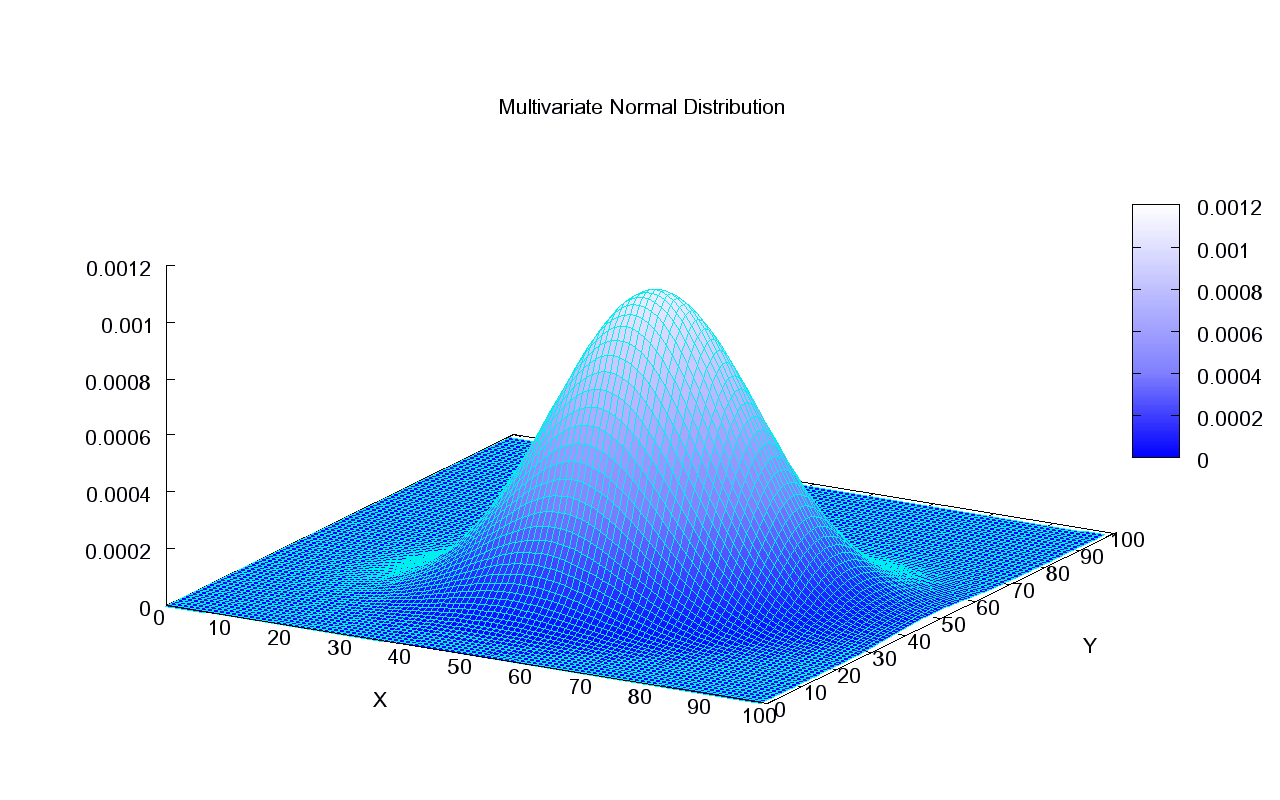
\includegraphics[width=\textwidth]{Multivariate_Gaussian.png}
\end{figure}
\end{column}
\end{columns}
\end{frame}

\begin{frame}{Multivariate Normal Distribution}
\begin{theorem}
$\mathbf{Y}\sim\mathcal{N}_n(\boldsymbol\mu, \boldsymbol\Sigma)$, and $\rank\boldsymbol\Sigma=n$\quad$\Rightarrow$\quad The pdf of $\mathbf{Y}$ has the form
$$
f_{\mathbf{Y}}(\mathbf{y})=\frac{1}{\sqrt{\det\boldsymbol{\Sigma}}(\sqrt{2\pi})^n}e^{-\frac12(\mathbf{y}-\boldsymbol\mu)^\top\boldsymbol{\Sigma}^{-1}(\mathbf{y}-\boldsymbol{\mu})}.
$$
\end{theorem}
\begin{block}{Proof.}
$\mathbf{Y}\sim\mathcal{N}_n(\boldsymbol\mu,\boldsymbol\Sigma)$\pause\quad$\Rightarrow$\quad$\exists\mathbf{A}\in\mathbb{R}^{n\times k},\,\mathbf{Z}\in\mathcal{N}_k(\mathbf{0},\mathbf{I}_k)$:
\pause$$
\mathbf{Y}=\mathbf{AZ}+\boldsymbol\mu\quad\text{with }\mathbf{AA}^\top=\boldsymbol\Sigma
$$
Since $n=\rank\boldsymbol\Sigma\pause=\rank\mathbf{AA}^\top\pause=k$, we have $k=n$.\\~\\
Also, $\det\boldsymbol\Sigma=\det\mathbf{AA}^\top=\det\mathbf{A}\cdot\det\mathbf{A}^\top=(\det\mathbf{A})^2$. Thus, 
$$\det\mathbf{A}=\sqrt{\det\boldsymbol\Sigma}.$$
\end{block}
\end{frame}

\begin{frame}{Multivariate Normal Distribution}
\begin{block}{Poof (cont'd).}
For the $\mathbf{Z}=\begin{bmatrix}
Z_1 & \cdots & Z_n
\end{bmatrix}$ with $Z_i\,\,{\stackrel{\text{iid}}{\sim}}\,\,\in\mathcal{N}(0,1)$,
\begin{align*}
f_{\mathbf{Z}}(\mathbf{z})\onslide<2->{&=f_{Z_1,\ldots,Z_n}(z_1,\ldots,z_n)}\onslide<3->{=\prod_{i=1}^n f_{Z_i}(z_i)}\onslide<4->{=\prod_{i=1}^n\frac{1}{\sqrt{2\pi}}e^{-\frac{z_i^2}{2}}\\}
\onslide<5->{&=\frac{1}{(\sqrt{2\pi})^n}e^{-\frac12(z_1^2+\ldots+z_n^2)}}\onslide<6->{=\frac{1}{(\sqrt{2\pi})^n}e^{-\frac12\mathbf{z}^\top\mathbf{z}}}
\end{align*}
\onslide<7->{Since $\mathbf{Y}=\mathbf{AZ}+\boldsymbol\mu$, and $\boldsymbol\Sigma=\mathbf{AA}^\top$, we have}
\begin{align*}
\onslide<8->{f_\mathbf{Y}(\mathbf{y})&=\frac{1}{\det\mathbf{A}}f_{\mathbf{Z}}(\mathbf{A}^{-1}(\mathbf{y}-\boldsymbol\mu))}\onslide<9->{=\frac{1}{\sqrt{\det\boldsymbol\Sigma}(\sqrt{2\pi})^n}e^{-\frac12(\mathbf{y}-\boldsymbol\mu)^\top(\mathbf{A}^{-1})^\top\mathbf{A}^{-1}(\mathbf{y}-\boldsymbol\mu)}\\}
\onslide<10->{&=\frac{1}{\sqrt{\det\boldsymbol\Sigma}(\sqrt{2\pi})^n}e^{-\frac12(\mathbf{y}-\boldsymbol\mu)^\top(\mathbf{A}^{\top})^{-1}\mathbf{A}^{-1}(\mathbf{y}-\boldsymbol\mu)}\\}
\onslide<11->{&=\frac{1}{\sqrt{\det\boldsymbol\Sigma|}(\sqrt{2\pi})^n}e^{-\frac12(\mathbf{y}-\boldsymbol\mu)^\top\boldsymbol\Sigma^{-1}(\mathbf{y}-\boldsymbol\mu)}}
\end{align*}
\end{block}
\end{frame}




\begin{frame}{Orthogonal Transform of a Multivariate Gaussian}
\begin{theorem}
Let $\mathbf{Z}\sim\mathcal{N}_n(\mathbf{0},\mathbf{I})$, and $\mathbf{Q}$ be an orthogonal $n\times n$ matrix ($\mathbf{Q}\in\mathcal{O}_n$). Then $\mathbf{QZ}\sim\mathcal{N}_n(\mathbf{0},\mathbf{I})$.
\end{theorem}
\begin{proof}
\onslide<2->{The pdf of $\mathbf{QZ}$ is}
\begin{align*}
\onslide<3->{f_{\mathbf{QZ}}(\mathbf{w})}\onslide<4->{&=\frac{1}{|\det\mathbf{Q}|}f_{\mathbf{Z}}(\mathbf{Q}^{-1}\mathbf{w})}\onslide<5->{=\frac{1}{1}\cdot\frac{1}{(\sqrt{2\pi})^n}e^{-\frac12(\mathbf{Q}^{-1}\mathbf{w})^\top(\mathbf{Q}^{-1}\mathbf{w})}\\}
\onslide<6->{&=\frac{1}{(\sqrt{2\pi})^n}e^{-\frac12(\mathbf{Q}^\top\mathbf{w})^\top(\mathbf{Q}^\top\mathbf{w})}}\onslide<7->{=\frac{1}{(\sqrt{2\pi})^n}e^{-\frac12(\mathbf{w}^\top\mathbf{Q})(\mathbf{Q}^\top\mathbf{w})}\\}
\onslide<8->{&=\frac{1}{(\sqrt{2\pi})^n}e^{-\frac12\mathbf{w}^\top(\mathbf{Q}\mathbf{Q}^\top)\mathbf{w}}}\onslide<9->{=\frac{1}{(\sqrt{2\pi})^n}e^{-\frac12\mathbf{w}^\top\mathbf{w}}}
\end{align*}
\onslide<10->{Hence, $\mathbf{QZ}\sim\mathcal{N}_n(\mathbf{0},\mathbf{I})$.}
\end{proof}
\end{frame}

\begin{frame}{Linear Transform of a Multivariate Gaussian}
\begin{theorem}
Let $\mathbf{Y}\sim\mathcal{N}_n(\boldsymbol\mu,\boldsymbol\Sigma)$. If $\mathbf{A}\in\mathbb{R}^{m\times n}$ with $\rank\mathbf{A}={\min}(m,n)$, then 
$$
\mathbf{AY}\sim\mathcal{N}_m(\mathbf{A}\boldsymbol\mu,\mathbf{A}\boldsymbol\Sigma\mathbf{A}^\top)
$$
\end{theorem}
\begin{proof}
Since $\mathbf{Y}\sim\mathcal{N}_n(\boldsymbol\mu,\boldsymbol\Sigma)$, we can write 
$$
\mathbf{Y}=\mathbf{BZ}+\boldsymbol\mu,
$$ 
\pause where $\mathbf{B}\in\mathbb{R}^{n\times k}$, $\mathbf{Z}\sim\mathcal{N}_{k}(\mathbf{0},\mathbf{I})$, and $\mathbf{BB}^\top=\boldsymbol\Sigma$. \pause Thus,
$$\mathbf{AY}=(\mathbf{AB})\mathbf{Z}+\mathbf{A}\boldsymbol\mu,$$ 
\pause where $\mathbf{AB}\in\mathbb{R}^{m\times k}$ s.t. $(\mathbf{AB})(\mathbf{AB})^\top=\mathbf{ABB}^\top\mathbf{A}=\mathbf{A}\boldsymbol\Sigma\mathbf{A}^\top$.
\end{proof}
\end{frame}

\iffalse
\begin{frame}{Multivariate Gaussian}{Uncorrelated Components are Independent}
\begin{theorem}
Let $\mathbf{y}\sim\mathcal{N}(\boldsymbol\mu,\boldsymbol\Sigma)$. Then $Y_i$ and $Y_j$ are independent\quad $\Leftrightarrow$ \quad $\Cov[Y_i,Y_j]=0$.
\end{theorem}
\begin{proof}
\vspace{150pt}
\end{proof}
\end{frame}
\fi

\section{Quadratic Forms of Multivariate Gaussians}

\begin{frame}{Non-central $\chi^2$ distribution}
\begin{definition}
Let $Y_i\,\,{\stackrel{\text{ind}}{\sim}}\,\,\mathcal{N}(\mu_i,1)$, \pause then the random variable
$$
\sum_{i=1}^n Y_i^2
$$
is said to have \textbf{noncentral chi-square} distribution with parameters $n$ and $\lambda=\sum_{i=1}^n\mu_i^2$.
\end{definition}
\vspace{-10pt}
\pause \begin{notation}
$\chi^2_{n}(\lambda)$
\end{notation}
\begin{itemize}
    \item\pause $n$ is called \textit{degrees of freedom}
    \item\pause $\lambda$ is called \textit{noncentrality parameter}
\end{itemize}
\vspace{-10pt}
\pause\begin{remark} Using matrix notation, if $\mathbf{Y}\sim\mathcal{N}_n(\boldsymbol\mu,\mathbf{I})$,\pause then $\mathbf{Y}^\top\mathbf{Y}\sim\chi^2_n(\lambda)$, with $\lambda=\boldsymbol\mu^\top\boldsymbol\mu$.
\end{remark}
\end{frame}


\begin{frame}{Quadratic Form of a Multivariate Gaussian}
\begin{theorem}
Let $\mathbf{Z}\sim\mathcal{N}_n(\mathbf{0},\mathbf{I})$, and $\mathbf{A}\in\mathbb{R}^{n\times n}$ be symmetric idempotent with $\rank\mathbf{A}=r$. Then
$\mathbf{Z}^\top\mathbf{A}\mathbf{Z}\sim\chi^2_r$.
\end{theorem}
\begin{proof}\begin{footnotesize}
\pause$\mathbf{A}^2=\mathbf{AA}=\mathbf{A}$. \pause Let $\mathbf{x}$ be an eigenvector of $\mathbf{A}$ and $\lambda$ is the corresponding eigenvalue. Then
$$
\mathbf{A}^2\mathbf{x}=\mathbf{AAx}\pause=\mathbf{A}\lambda\mathbf{x}=\lambda\mathbf{Ax}\pause=\lambda^2\mathbf{x}\pause=\lambda\mathbf{x}=\mathbf{Ax}
$$
\pause So, $(\lambda^2-\lambda)\mathbf{x}=\mathbf{0}\pause\quad\Rightarrow\quad\lambda^2-\lambda=0\quad\Rightarrow\quad\lambda\in\{0,1\}$.\\~\\

\pause Eigendecomposition of $\mathbf{A}$: \pause $\mathbf{A}=\mathbf{Q}^\top\boldsymbol\Lambda\mathbf{Q}$, \pause where $\boldsymbol\Lambda=\mathrm{diag}(\underbrace{1,\ldots,1}_{r},\underbrace{0,\ldots,0}_{n-r})$.\\~\\

Thus, $\mathbf{Z}^\top\mathbf{AZ}\pause=\mathbf{Z}^\top\mathbf{Q}^\top\boldsymbol\Lambda\mathbf{Q}\mathbf{Z}\pause=(\mathbf{QZ})^\top\boldsymbol\Lambda(\mathbf{QZ})\pause=\tilde{\mathbf{Z}}^\top\boldsymbol\Lambda\tilde{\mathbf{Z}}\pause=\sum_{i=1}^r\tilde{Z}_i^2\sim\chi^2_r$, \pause where $\tilde{\mathbf{Z}}=(\tilde{Z}_1,\ldots,\tilde{Z}_n)\sim\mathcal{N}_n(\mathbf{0},\mathbf{I})$.
\end{footnotesize}
\end{proof}
\end{frame}


\begin{frame}{Quadratic Form of a Multivariate Gaussian}
\begin{theorem}
Let $\mathbf{Y}\sim\mathcal{N}_n(\boldsymbol\mu,\mathbf{I})$, and $\mathbf{A}\in\mathbb{R}^{n\times n}$ be symmetric idempotent with $\rank\mathbf{A}=r$. Then
$\mathbf{Y}^\top\mathbf{A}\mathbf{Y}\sim\chi^2_r(\lambda)$, with $\lambda=\boldsymbol\mu^\top\mathbf{A}\boldsymbol\mu$
\end{theorem}
\begin{proof}
\pause $\mathbf{A}=\mathbf{Q}^\top\boldsymbol\Lambda\mathbf{Q}$, where $\boldsymbol\Lambda=\mathrm{diag}(1,\ldots,1,0,\ldots,0)$. \pause Thus,
$$
\mathbf{Y}^\top\mathbf{AY}=(\mathbf{QY})^\top\boldsymbol\Lambda(\mathbf{QY})
$$
\pause Notice that $\tilde{\mathbf{Y}}:=\mathbf{QY}\sim\mathcal{N}_n(\mathbf{Q}\boldsymbol\mu,\mathbf{I})$. (Why?) \pause Therefore,
$$
\mathbf{Y}^\top\mathbf{AY}=\tilde{\mathbf{Y}}^\top\boldsymbol\Lambda\tilde{\mathbf{Y}}=\sum_{i=1}^r\tilde{Y}_i^2\sim\chi^2_r(\lambda),
$$
\pause where $\lambda=(\boldsymbol\Lambda\mathbf{Q}\boldsymbol\mu)^\top(\boldsymbol\Lambda\mathbf{Q}\boldsymbol\mu)=\boldsymbol\mu^\top\mathbf{Q}^\top\boldsymbol\Lambda^\top\boldsymbol\Lambda\mathbf{Q}\boldsymbol\mu=\boldsymbol\mu^\top\mathbf{Q}^\top\boldsymbol\Lambda\mathbf{Q}\boldsymbol\mu$\\
$=\boldsymbol\mu^\top\mathbf{A}\boldsymbol\mu$.
\end{proof}
\end{frame}

\iffalse
\begin{frame}{Quadratic Form of a Multivariate Gaussian}
\begin{theorem}
Let $\mathbf{Y}\sim\mathcal{N}_n(\boldsymbol\mu,\boldsymbol\Sigma)$, $\boldsymbol\Sigma\succ\mathbf{0}$, $\mathbf{A}\boldsymbol\Sigma$ be idempotent matrix, and  $\rank(\mathbf{A})=r$. Then $\mathbf{Y}^\top\mathbf{AY}\sim\chi^2_r(\lambda)$ with $\lambda=\boldsymbol\mu^\top\mathbf{A}\boldsymbol\mu$.
\end{theorem}
\begin{proof}\begin{footnotesize}
\pause $\mathbf{Y}\sim\mathcal{N}_n(\boldsymbol\mu,\boldsymbol{\Sigma})\quad\Rightarrow\quad\tilde{\mathbf{Y}}:={\boldsymbol\Sigma}^{-1/2}\mathbf{Y}\sim\mathcal{N}_n(\boldsymbol\Sigma^{-1/2}\boldsymbol\mu,\mathbf{I})$\qquad (Why?).\pause\quad Also,
\begin{equation}
\mathbf{Y}^\top\mathbf{AY}=\mathbf{Y}^\top\boldsymbol\Sigma^{-1/2}\boldsymbol\Sigma^{1/2}\mathbf{A}\boldsymbol\Sigma^{1/2}\boldsymbol\Sigma^{-1/2}\mathbf{Y}=\tilde{\mathbf{Y}}^\top(\boldsymbol\Sigma^{1/2}\mathbf{A}\boldsymbol\Sigma^{1/2})\tilde{\mathbf{Y}}\label{eq:decor}    
\end{equation}
\pause We are given that $\mathbf{A}\boldsymbol\Sigma\mathbf{A}\boldsymbol\Sigma=\mathbf{A}\boldsymbol\Sigma$, thus $\mathbf{A}\boldsymbol\Sigma\mathbf{A}=\mathbf{A}$, and 
\pause $$(\boldsymbol\Sigma^{1/2}\mathbf{A}\boldsymbol\Sigma^{1/2})(\boldsymbol\Sigma^{1/2}\mathbf{A}\boldsymbol\Sigma^{1/2})\pause=\boldsymbol\Sigma^{1/2}\mathbf{A}\boldsymbol\Sigma\mathbf{A}\boldsymbol\Sigma^{1/2}\pause=\boldsymbol\Sigma^{1/2}\mathbf{A}\boldsymbol\Sigma^{1/2}$$%
\pause Thus, $\tilde{\mathbf{A}}:=\boldsymbol\Sigma^{1/2}\mathbf{A}\boldsymbol\Sigma^{1/2}$ is idempotent, and its rank is $r$ (check this). \pause Combining this with \eqref{eq:decor}, we have
$$
\mathbf{Y}^\top\mathbf{AY}\pause=\tilde{\mathbf{Y}}^\top\tilde{\mathbf{A}}\tilde{\mathbf{Y}}\sim\chi^2_r(\lambda)
$$
\pause with $\lambda=(\boldsymbol\Sigma^{-1/2}\boldsymbol\mu)^\top(\boldsymbol\Sigma^{1/2}\mathbf{A}\boldsymbol\Sigma^{1/2})(\boldsymbol\Sigma^{-1/2}\boldsymbol\mu)=\boldsymbol\mu^\top\mathbf{A}\boldsymbol\mu$.
\end{footnotesize}
\end{proof}
\end{frame}
\fi

\begin{frame}{Matrix Calculus}
It is useful to have differentiation rules for matrix and vector expressions. \onslide<2->{The most important for our purposes are
\begin{align*}
&\boldsymbol{\nabla}_\mathbf{x}(\mathbf{a}^\top\mathbf{x})=\mathbf{a}\\
&\boldsymbol{\nabla}_\mathbf{x}(\mathbf{x}^\top\mathbf{Ax})=(\mathbf{A}+\mathbf{A}^\top)\mathbf{x}
\end{align*}
}%
\onslide<3->{Note that the second rule is defined only if $\mathbf{A}$ is square. Furthermore, if $\mathbf{A}$ is symmetric, we can simplify the result to $2\mathbf{Ax}$.}
\onslide<4->{\begin{exe}
Prove the rules above.
\end{exe}}
\end{frame}

\begin{frame}{Back to SLR}
Recall the SLR in matrix form:
$$
\mathbf{Y}\sim\mathcal{N}_n(\mathbf{X}\boldsymbol\beta,\sigma^2\mathbf{I})
$$
\pause Least squares objective is
\begin{align*}
\onslide<2->{Q(\beta_0,\beta_1)&=\sum_{i=1}^n[Y_i-(\beta_0+\beta_1 x_i)]^2}\onslide<3->{=(\mathbf{Y}-\mathbf{X}\boldsymbol\beta)^\top(\mathbf{Y}-\mathbf{X}\boldsymbol\beta)\\}
\onslide<4->{&=\mathbf{Y}^\top\mathbf{Y}-\boldsymbol\beta^\top\mathbf{X}^\top\mathbf{Y}-\mathbf{Y}^\top\mathbf{X}\boldsymbol\beta+\boldsymbol\beta^\top\mathbf{X}^\top\mathbf{X}\boldsymbol\beta\\}
\onslide<5->{\nabla_{\boldsymbol\beta}Q&=\mathbf{X}^\top\mathbf{Y}-\mathbf{X}^\top\mathbf{Y}+2\mathbf{X}^\top\mathbf{X}\boldsymbol\beta}\onslide<6->{=2\mathbf{X}^\top\mathbf{X}\boldsymbol\beta-2\mathbf{X}^\top\mathbf{Y}}\onslide<7->{=\mathbf{0}\\}
\onslide<8->{&\mathbf{X}^\top\mathbf{X}\boldsymbol\beta=\mathbf{X}^\top\mathbf{Y}\quad\Rightarrow\quad}\onslide<9->{\boxed{\hat{\boldsymbol\beta}=(\mathbf{X}^\top\mathbf{X})^{-1}\mathbf{X}^\top\mathbf{Y}}}
\end{align*}
\onslide<10->{where we used  $\mathbf{X}^\top\mathbf{X}=\begin{bmatrix}
n & \sum_i x_i\\
\sum_i x_i & \sum_i x_i^2
\end{bmatrix}$ is non-singular (check).}\\~\\
\onslide<11->{The predictions are} $\onslide<11->{(\hat{Y}_1,\ldots,\hat{Y}_n)=\hat{\mathbf{Y}}=\mathbf{X}\hat{\boldsymbol\beta}}\onslide<12->{=\mathbf{X}(\mathbf{X}^\top\mathbf{X})^{-1}\mathbf{X}^\top\mathbf{Y}}$
\end{frame}

\section{Distributions of SSE, SSR; Independence}

\begin{frame}{Distribution of SSE}
\begin{theorem}
$\frac{\text{SSE}}{\sigma^2}\sim\chi^2_{n-2}$
\end{theorem}
\begin{block}{Proof.}\begin{small}
\vspace{-20pt}
\begin{align*}
\onslide<2->{\text{SSE}&=\sum_{i=1}^n(Y_i-\hat{Y}_i)^2}\onslide<3->{=(\mathbf{Y}-\hat{\mathbf{Y}})^\top(\mathbf{Y}-\hat{\mathbf{Y}})\\}
\onslide<4->{&=[\mathbf{Y}-\mathbf{X}(\mathbf{X}^\top\mathbf{X})^{-1}\mathbf{X}^\top\mathbf{Y}]^\top[\mathbf{Y}-\mathbf{X}(\mathbf{X}^\top\mathbf{X})^{-1}\mathbf{X}^\top\mathbf{Y}]\\}
\onslide<5->{&=\mathbf{Y}^\top[\mathbf{I}-\mathbf{X}(\mathbf{X}^\top\mathbf{X})^{-1}\mathbf{X}^\top]^\top[\mathbf{I}-\mathbf{X}(\mathbf{X}^\top\mathbf{X})^{-1}\mathbf{X}^\top]\mathbf{Y}}
\end{align*}
\onslide<6->{The matrix $\mathbf{A}:=\mathbf{I}-\mathbf{X}(\mathbf{X}^\top\mathbf{X})^{-1}\mathbf{X}^\top$ is symmetric (check) and idempotent:}
\begin{align*}
\onslide<7->{\mathbf{A}^2&=[\mathbf{I}-\mathbf{X}(\mathbf{X}^\top\mathbf{X})^{-1}\mathbf{X}^\top][\mathbf{I}-\mathbf{X}(\mathbf{X}^\top\mathbf{X})^{-1}\mathbf{X}^\top]\\}
\onslide<8->{&=\mathbf{I}-2\mathbf{X}(\mathbf{X}^\top\mathbf{X})^{-1}\mathbf{X}^\top+\mathbf{X}(\mathbf{X}^\top\mathbf{X})^{-1}\mathbf{X}^\top\mathbf{X}(\mathbf{X}^\top\mathbf{X})^{-1}\mathbf{X}^\top\\}
\onslide<9->{&=\mathbf{I}-\mathbf{X}(\mathbf{X}^\top\mathbf{X})^{-1}\mathbf{X}^\top=\mathbf{A}}
\end{align*}
\onslide<10->{Hence, $\text{SSE}=\mathbf{Y}^\top\mathbf{A}^\top\mathbf{AY}=\mathbf{Y}^\top\mathbf{A}\mathbf{Y}$.}
\end{small}\end{block}
\end{frame}

\begin{frame}{Distribution of SSE}
\begin{proof}[Proof (cont'd).]
Recall, $\mathbf{Y}\sim\mathcal{N}_n(\mathbf{X}\boldsymbol\beta,\sigma^2\mathbf{I})$\pause\quad$\Rightarrow$\quad$\sigma^{-1}\mathbf{Y}\sim\mathcal{N}_n(\sigma^{-1}\mathbf{X}\boldsymbol\beta,\mathbf{I})$. \pause Hence, 
\begin{align*}
\onslide<3->{\frac{\text{SSE}}{\sigma^2}&=(\sigma^{-1}\mathbf{Y})^\top\mathbf{A}(\sigma^{-1}\mathbf{Y})\pause}\onslide<4->{\sim\chi^2_{\rank\mathbf{A}}(\lambda),\\}
\onslide<5->{\text{where\quad }\rank\mathbf{A}&=\trace\mathbf{A}}\onslide<6->{=\trace[\mathbf{I}-\mathbf{X}(\mathbf{X}^\top\mathbf{X})^{-1}\mathbf{X}^\top]\\}
\onslide<7->{&=\trace\mathbf{I}-\trace[\mathbf{X}(\mathbf{X}^\top\mathbf{X})^{-1}\mathbf{X}^\top]\\}
\onslide<8->{&=n-\trace[(\mathbf{X}^\top\mathbf{X})^{-1}\mathbf{X}^\top\mathbf{X}]}\onslide<9->{=n-2,\\}
\onslide<10->{\text{and\quad }\lambda&=(\sigma^{-1}\mathbf{X}\boldsymbol\beta)^\top\mathbf{A}(\sigma^{-1}\mathbf{X}\boldsymbol\beta)\\}
\onslide<11->{&=\frac1{\sigma^2}\boldsymbol\beta^\top\mathbf{X}^\top[\mathbf{I}-\mathbf{X}(\mathbf{X}^\top\mathbf{X})^{-1}\mathbf{X}^\top]\mathbf{X}\boldsymbol\beta\\}
\onslide<12->{&=\frac{1}{\sigma^2}\boldsymbol\beta^\top[\mathbf{X}^\top\mathbf{X}-\mathbf{X}^\top\mathbf{X}(\mathbf{X}^\top\mathbf{X})^{-1}\mathbf{X}^\top\mathbf{X}]\boldsymbol\beta}\onslide<13->{=0}
\end{align*}
\onslide<14->{Finally, $\frac{\text{SSE}}{\sigma^2}\sim\chi^2_{n-2}$.}
\end{proof}    
\end{frame}

\begin{frame}{Distribution of SSR}
\begin{theorem}
$\frac{\text{SSR}}{\sigma^2}\sim\chi^2_1$ (non-central)
\end{theorem}
\begin{block}{Proof.}\begin{small}
\onslide<2->{Let $\mathbf{1}:=(1,\ldots,1)$, then $\mathbf{1}^\top\mathbf{1}=n$}\onslide<3->{, and $\bar{Y}=\frac{\mathbf{1}^\top\mathbf{Y}}{\mathbf{1}^\top\mathbf{1}}$.\\~\\}
\onslide<4->{Let $\bar{\mathbf{Y}}:=(\bar{Y},\ldots,\bar{Y})$. Then $\bar{\mathbf{Y}}=\mathbf{1}(\mathbf{1}^\top\mathbf{1})^{-1}\mathbf{1}^\top\mathbf{Y}$}
\begin{align*}
\onslide<5->{\text{SSR}&=\sum_{i=1}^n(\hat{Y}_i-\bar{Y})^2}\onslide<6->{=(\hat{\mathbf{Y}}-\bar{\mathbf{Y}})^\top(\hat{\mathbf{Y}}-\bar{\mathbf{Y}})\\}
\onslide<7->{&=[\mathbf{X}(\mathbf{X}^\top\mathbf{X})^{-1}\mathbf{X}^\top\mathbf{Y}-\mathbf{1}(\mathbf{1}^\top\mathbf{1})^{-1}\mathbf{1}^\top\mathbf{Y}]^\top[\mathbf{X}(\mathbf{X}^\top\mathbf{X})^{-1}\mathbf{X}^\top\mathbf{Y}-\mathbf{1}(\mathbf{1}^\top\mathbf{1})^{-1}\mathbf{1}^\top\mathbf{Y}]\\}
\onslide<8->{&=\mathbf{Y}^\top[\mathbf{X}(\mathbf{X}^\top\mathbf{X})^{-1}\mathbf{X}^\top-\mathbf{1}(\mathbf{1}^\top\mathbf{1})^{-1}\mathbf{1}^\top]^\top[\mathbf{X}(\mathbf{X}^\top\mathbf{X})^{-1}\mathbf{X}^\top-\mathbf{1}(\mathbf{1}^\top\mathbf{1})^{-1}\mathbf{1}^\top]\mathbf{Y}}
\end{align*}
\onslide<9->{The matrix $\mathbf{B}:=\mathbf{X}(\mathbf{X}^\top\mathbf{X})^{-1}\mathbf{X}^\top-\mathbf{1}(\mathbf{1}^\top\mathbf{1})^{-1}\mathbf{1}^\top$ is symmetric and idempotent (check).}
\onslide<10->{Hence, $\text{SSR}=\mathbf{Y}^\top\mathbf{B}^\top\mathbf{BY}=\mathbf{Y}^\top\mathbf{B}\mathbf{Y}$.}
\end{small}\end{block}
\end{frame}

\begin{frame}{Distribution of SSR}
\begin{proof}[Proof (cont'd).]
Recall, $\mathbf{Y}\sim\mathcal{N}_n(\mathbf{X}\boldsymbol\beta,\sigma^2\mathbf{I})$\pause\quad$\Rightarrow$\quad$\sigma^{-1}\mathbf{Y}\sim\mathcal{N}_n(\sigma^{-1}\mathbf{X}\boldsymbol\beta,\mathbf{I})$. \pause Hence, 
\begin{align*}
\onslide<3->{\frac{\text{SSR}}{\sigma^2}&=(\sigma^{-1}\mathbf{Y})^\top\mathbf{B}(\sigma^{-1}\mathbf{Y})\pause}\onslide<4->{\sim\chi^2_{\rank\mathbf{B}}(\lambda),\\}
\onslide<5->{\text{where\quad }\rank\mathbf{B}&=\trace\mathbf{B}}\onslide<6->{=\trace[\mathbf{X}(\mathbf{X}^\top\mathbf{X})^{-1}\mathbf{X}^\top-\mathbf{1}(\mathbf{1}^\top\mathbf{1})^{-1}\mathbf{1}^\top]\\}
\onslide<7->{&=\trace[\mathbf{X}(\mathbf{X}^\top\mathbf{X})^{-1}\mathbf{X}^\top]-\trace[\mathbf{1}(\mathbf{1}^\top\mathbf{1})^{-1}\mathbf{1}^\top]\\}
\onslide<8->{&=\trace[(\mathbf{X}^\top\mathbf{X})^{-1}\mathbf{X}^\top\mathbf{X}]-\trace[(\mathbf{1}^\top\mathbf{1})^{-1}\mathbf{1}^\top\mathbf{1}]\\}
\onslide<9->{&=\trace\mathbf{I}_2-\trace1=2-1=1\\}
\end{align*}
\onslide<10->{Finally, $\frac{\text{SSR}}{\sigma^2}\sim\chi^2_{1}$ (non-central).}
\end{proof}    
\end{frame}

\begin{frame}{Independence between SSR and SSE}
\begin{theorem}
Let $\mathbf{Y}\sim\mathcal{N}_n(\boldsymbol\mu,\boldsymbol\Sigma)$, and $\boldsymbol\Sigma\succ\mathbf{0}$. Then two quadratic forms $\mathbf{Y}^\top\mathbf{A}\mathbf{Y}$ and $\mathbf{Y}^\top\mathbf{BY}$ are independent \quad$\Leftrightarrow$\quad $\mathbf{A}\boldsymbol\Sigma\mathbf{B}=\mathbf{0}$.
\end{theorem}    

\pause\begin{theorem}
SSR and SSE are independent.
\end{theorem}
\begin{proof}
\pause $\text{SSE}=\mathbf{Y}^\top\mathbf{A}\mathbf{Y}$ with $\mathbf{A}=\mathbf{I}-\mathbf{X}(\mathbf{X}^\top\mathbf{X})^{-1}\mathbf{X}^\top$\\
\pause $\text{SSR}=\mathbf{Y}^\top\mathbf{B}\mathbf{Y}$ with $\mathbf{B}=\mathbf{X}(\mathbf{X}^\top\mathbf{X})^{-1}\mathbf{X}^\top-\mathbf{1}(\mathbf{1}^\top\mathbf{1})^{-1}\mathbf{1}^\top$\\
\pause $\mathbf{Y}\sim\mathcal{N}_n(\mathbf{X}\boldsymbol\beta,\sigma^2\mathbf{I})$. \pause And now let's check
\begin{align*}
\onslide<6->{&\mathbf{A}\sigma^2\mathbf{IB}=\sigma^2\mathbf{AB}\\}
\onslide<7->{&=\sigma^2[\mathbf{I}-\mathbf{X}(\mathbf{X}^\top\mathbf{X})^{-1}\mathbf{X}^\top][\mathbf{X}(\mathbf{X}^\top\mathbf{X})^{-1}\mathbf{X}^\top-\mathbf{1}(\mathbf{1}^\top\mathbf{1})^{-1}\mathbf{1}^\top]\\}
\onslide<8->{&=\sigma^2[\mathbf{X}(\mathbf{X}^\top\mathbf{X})^{-1}\mathbf{X}^\top-\mathbf{X}(\mathbf{X}^\top\mathbf{X})^{-1}\mathbf{X}^\top-\mathbf{1}(\mathbf{1}^\top\mathbf{1})^{-1}\mathbf{1}^\top\mathbf{X}(\mathbf{X}^\top\mathbf{X})^{-1}\mathbf{X}^\top]\\}
\onslide<9->{&=\mathbf{0}}
\end{align*}
\onslide<10->{Hence, SSE and SSR are independent.}
\end{proof}

\end{frame}

\end{document}